\documentclass[../../main.tex]{subfiles}


\begin{document}
\subsection*{(a)}
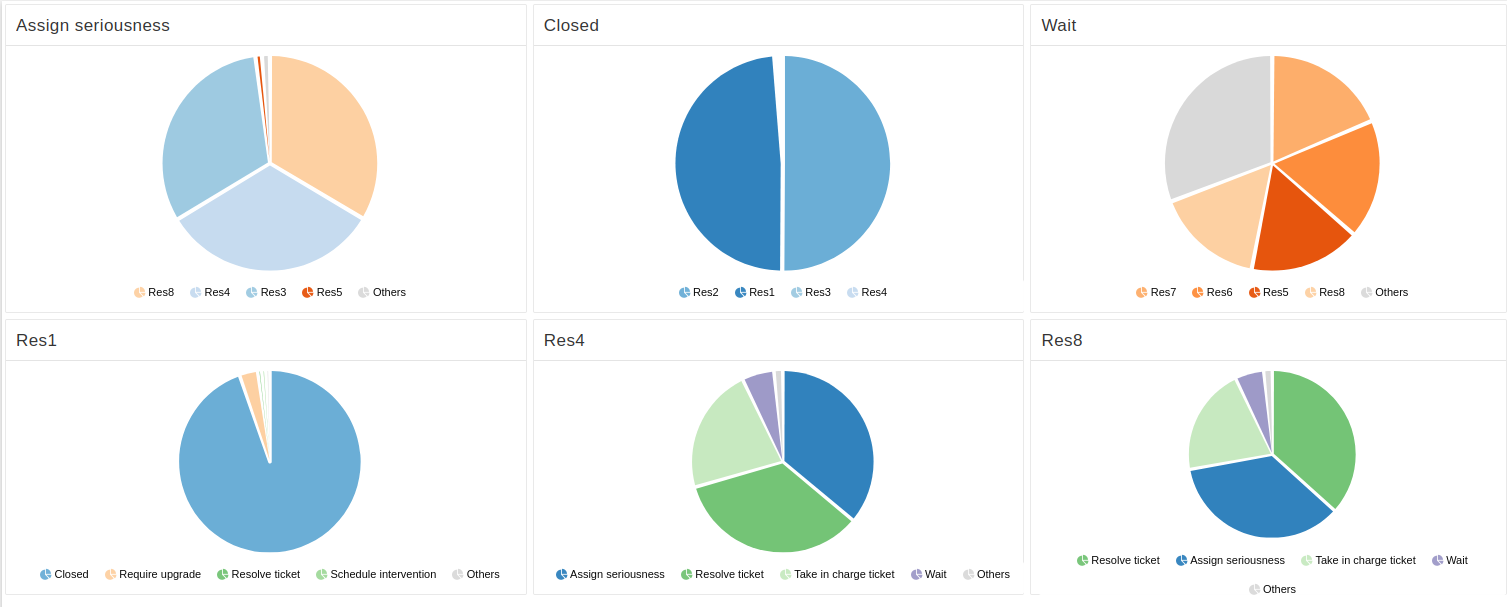
\includegraphics[width=\columnwidth]{img/Celonis_a_Visualization.png}\\
For the left Pie Chart we used \verb|"event_table_csv"."RESOURCE"| as the Dimension and \verb|COUNT("event_table_csv"."ACTIVITY")| as the KPI.\\
For the right Pie Chart we used \verb|"event_table_csv"."ACTIVITY"| as the Dimension and \verb|COUNT("event_table_csv"."RESOURCE")| as the KPI.


\subsection*{(b)}
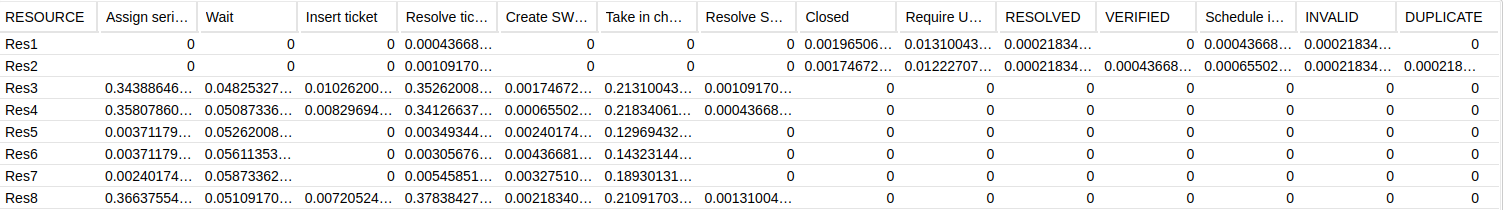
\includegraphics[width=\columnwidth]{img/Celonis_b_OLAP.png}\\
\begin{verbatim}
	SOURCE("event_table_csv"."RESOURCE")
\end{verbatim}
\begin{lstlisting}
	SUM(CASE WHEN SOURCE ( "event_table_csv"."ACTIVITY" ) = '[ACTIVITY]' THEN 1 ELSE 0 END) / 4580
\end{lstlisting}
Replace \verb|[ACTIVITY]| with each of the 14 Activities for the corresponding Dimensions. 4580 is the number of cases obtained by \verb|COUNT_TABLE("case_table_csv")|.

\subsection*{(c)}
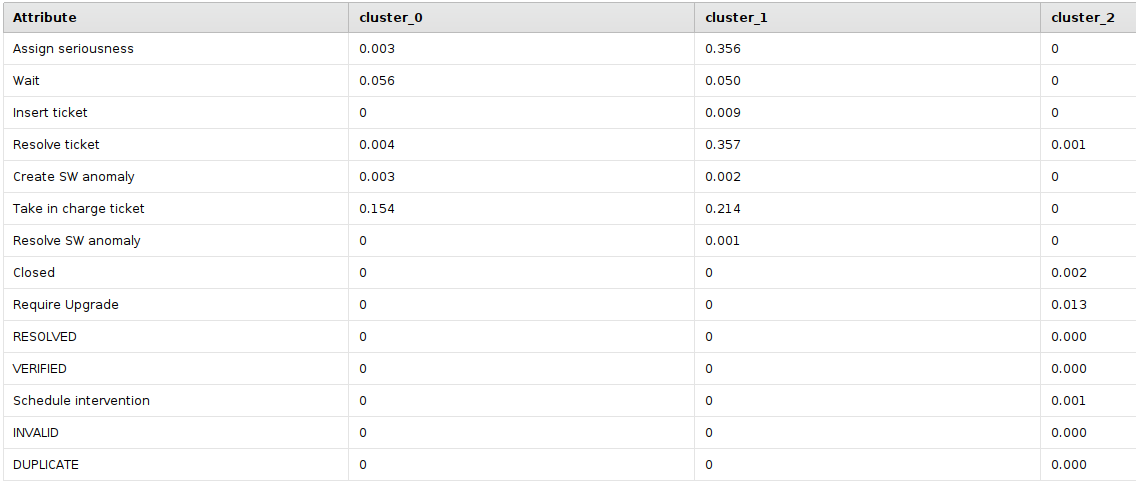
\includegraphics[width=0.75\columnwidth]{img/RapidMiner_c_Centriods.png}
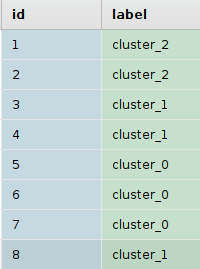
\includegraphics[width=0.25\columnwidth]{img/RapidMiner_c_Clustering.png}\\
We observed that Resources 3,4,8 were the only ones that executed 'Insert Ticket' and 'Resolve SW anomaly', thus forming cluster 1, which's centroid also reflects this. Resources 1,2 were the only ones to close any tickets (amongst other Activities), forming cluster 2. Resources 5,6,7 did none of these Activities, but also called Activities that Resources in cluster 1 called.


\subsection*{(d)}
\includegraphics[width=\columnwidth]{img/Celonis_d_OLAP.png}\\
\begin{verbatim}
	SOURCE("event_table_csv"."RESOURCE")
\end{verbatim}
\begin{verbatim}
	TARGET("event_table_csv"."RESOURCE")
\end{verbatim}
\begin{lstlisting}
	COUNT(SOURCE("event_table_csv"."ACTIVITY")) / 4580
\end{lstlisting}
4580 is the number of cases obtained by \verb|COUNT_TABLE("case_table_csv")|.

\subsection*{(e)}
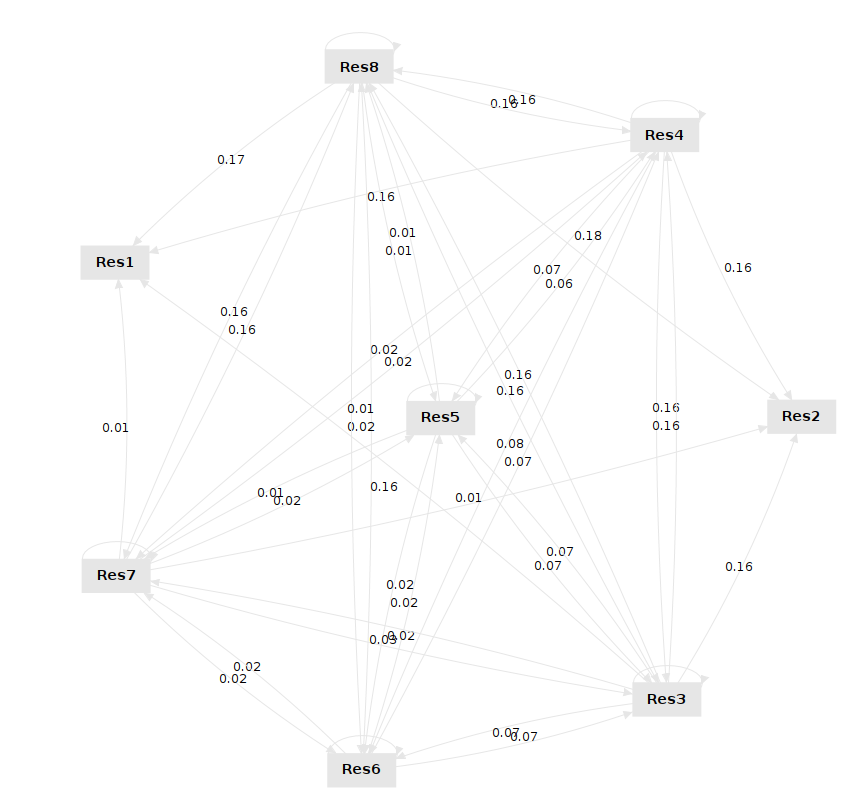
\includegraphics[width=\columnwidth]{img/RapidMiner_e_Graph.png}

\subsection*{(f)}

\subsection*{(g)}

\end{document}